\documentclass[12pt]{article}
\usepackage[utf8]{inputenc}
\usepackage{geometry}
\geometry{margin=1in}
\usepackage{amsmath}
\usepackage{tikz}
\usepackage{pgfplots}
\pgfplotsset{compat=1.15}

\title{Island Economy Exercise}
\author{Macroeconomics \\  Scarcity and Choice}
\date{}

\begin{document}
\maketitle

\noindent \textbf{Group Members:} \underline{\hspace{10cm}}

\section*{Part A: Scarcity and Trade-Offs (Round 1)}
Your group has \textbf{10 resource tokens}. You can allocate them to produce \textbf{Fish} or \textbf{Shelters}:
\begin{itemize}
    \item 1 token = 1 Fish
    \item 2 tokens = 1 Shelter
\end{itemize}

\noindent \textbf{Decision:}
\begin{itemize}
    \item Fish Produced: \underline{\hspace{2cm}}
    \item Shelters Produced: \underline{\hspace{2cm}}
\end{itemize}

\noindent \textbf{Questions:}
\begin{enumerate}
    \item What trade-off did you face when allocating tokens?
    \item If you wanted 1 more shelter, what would you have to give up? (Opportunity Cost)
\end{enumerate}

\section*{Part B: Production Possibilities Frontier (PPF)}
Use the graph below to plot all possible combinations of Fish and Shelters your group could produce with 10 tokens.

\[
\text{Example: 0 Shelters $\to$ 10 Fish; 1 Shelter $\to$ 8 Fish; etc.}
\]

\begin{center}
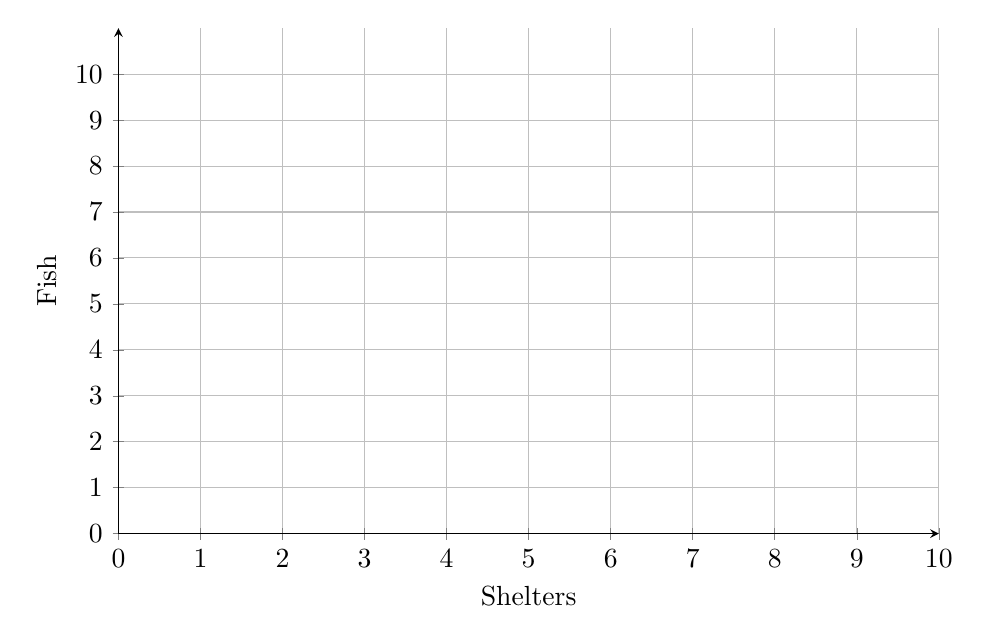
\begin{tikzpicture}
\begin{axis}[
    width=12cm, height=8cm,
    axis lines=left,
    xlabel={Shelters},
    ylabel={Fish},
    xmin=0, xmax=10,
    ymin=0, ymax=11,
    xtick={0,...,10},
    ytick={0,1,...,10},
    grid=both
]
% Example PPF points (10 tokens)
%\addplot[mark=*, thick] coordinates {
   % (0,10) (1,8) (2,6) (3,4) (4,2) (5,0)
%};
\end{axis}
\end{tikzpicture}
\end{center}

\section*{Part C: Specialization and Trade (Round 2)}
Now, some groups have \textbf{Fishing Advantage} (1 token = 2 Fish), while others have \textbf{Shelter Advantage} (1 token = 1 Shelter). Work with another group to specialize and trade.

\noindent \textbf{Record Before Trade:}
\begin{itemize}
    \item Fish = \underline{\hspace{2cm}}, Shelters = \underline{\hspace{2cm}}
\end{itemize}

\noindent \textbf{Record After Trade:}
\begin{itemize}
    \item Fish = \underline{\hspace{2cm}}, Shelters = \underline{\hspace{2cm}}
\end{itemize}

\noindent \textbf{Questions:}
\begin{enumerate}
    \item How did specialization change your production?
    \item Did trade make your group better off? Why or why not?
\end{enumerate}

\section*{Part D: Economic Shocks (Round 3)}
Suppose a storm destroys half of all shelters on the island.
\begin{enumerate}
    \item How does this change the value of Fish vs. Shelters?
    \item If a new fishing net doubles fishing productivity, how does this shift the PPF?
\end{enumerate}

\section*{Reflection Questions}
\begin{enumerate}
    \item How does this exercise illustrate the concept of \textbf{scarcity}?
    \item How does the PPF show \textbf{opportunity costs}?
    \item Why do countries specialize and trade in the real world?
    \item What happens to an economy’s choices when technology or resources change?
\end{enumerate}

\end{document}
